We are using a ray casting method for rendering our fire. The ray caster collects temperatures over the scene and transform them into a color for each pixel using black-body radiation.
\section{Black-body radiation}
	To be able to convert a temperature sample in the grid to a color, we use the black-body radiation model. 


\begin{figure}[h!]
\label{fig:blackbody}
\centering
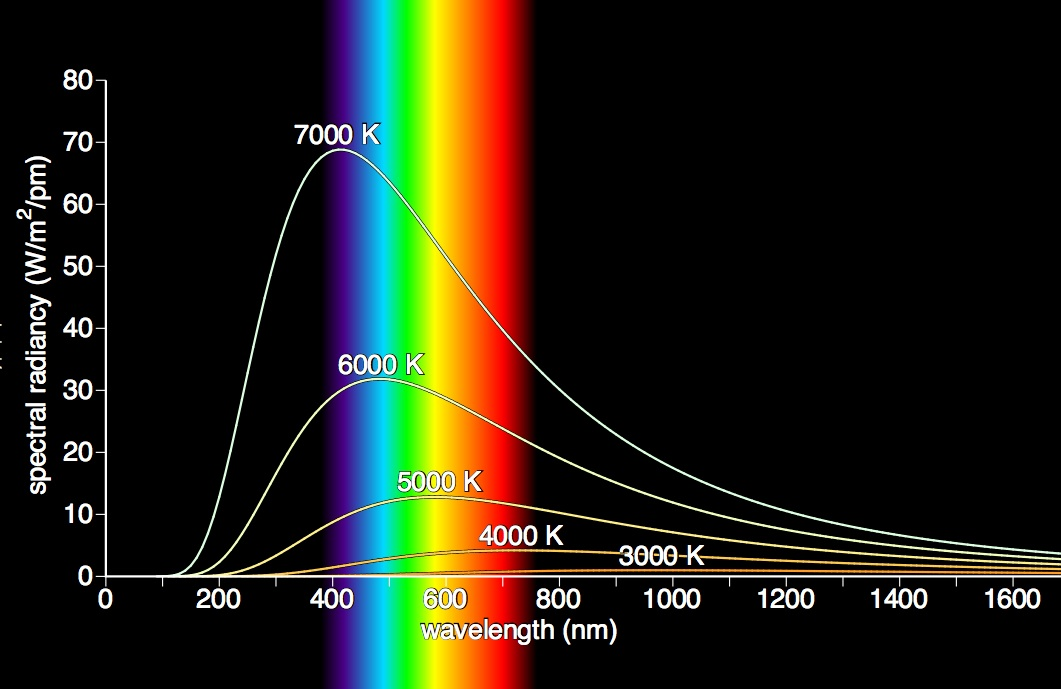
\includegraphics[width=0.6\textwidth]{blackbody.png}
\caption{Five different temperatures and their respective spectral radiancy depending on the wavelength. Notice the color spectrum that the human eye can observe, from 400 to 700 nm.}
\end{figure}

The black-body radiation model calculates an emitted radiance for a given wavelength and temperature, Planck's formula\cite{Nguyen02} equation \ref{eq:planck}. Where $C_1 \approx 3.7418 \cdot 10^{-16} Wm^2$ and $C_2 \approx 1.4388 \cdot 10^{-2} m^\circ K$

\begin{equation}
\label{eq:planck}
	L_{e,\lambda}(x) = \frac{2C_1}{\lambda^5(e^{C_2/(\lambda T)}-1)}
\end{equation}
This allows us to calculate the spectral radiance $L$ for a given wavelength $\lambda$ and position using the radiative transport, equation \ref{eq:blackbody}, using the blackbody radiation as the emitted radiance. 

\begin{equation}
\label{eq:blackbody}
\begin{split}
	(\vec{\omega}\cdot \nabla)L_\lambda(x,\vec{\omega}) = -\sigma_t(x)L_\lambda(x,\vec{\omega}) + \\ 
\sigma_s(x) \int_{4\pi} p(\vec{\omega},\vec{\omega}')L_\lambda(x,\vec{\omega}')d\vec{\omega}' + \\
\sigma_a(x)L_{e,\lambda}(x,)
\end{split}
\end{equation}
The scattering part, $ p(\vec{\omega},\vec{\omega}')$,  is neglected due to the high computation time and the fact that there are few scattering effects in flames. \\\\
The achieved radiance is then mapped onto the XYZ-color space by using the CIE standard observer 1931\cite{CIE}.
We then convert the XYZ colors to the LMS-color space with the CAT02 transformation method \cite{CAT02}, equation \ref{eq:3}.

\begin{equation}
\label{eq:3}
	\begin{bmatrix}
       L          \\
       M \\
       S
     \end{bmatrix} =
 	\begin{bmatrix}
       0.7328 & 0.4296 & -0.1624 \\
     -0.7036 & 1.6975 &  0.0061 \\
0.0030 & 0.0136 & 0.9834
     \end{bmatrix}
\begin{bmatrix}
      X          \\
       Y \\
       Z
     \end{bmatrix}
\end{equation}
We also add an chromatic adaption at this step to get a result as if the observers eyes and thereby vision have adapted to the intensity in the scene. Without this step a too bright flame was produced which is the case when looking at a flame with a normal to large sized pupil. \\\\
The LMS values are then converted back by inverting Equation 3. And finally the XYZ values are converted into the RGB-color space with an sRGB conversion, Equation \ref{eq:4} \cite{sRGB}.

\begin{equation}
\label{eq:4}
	\begin{bmatrix}
      R          \\
       G \\
       B
     \end{bmatrix} =
 	\begin{bmatrix}
      3.2410	& -1.5374	&  -0.4986 \\
	 -0.9692 & 1.8760	&  0.0416 \\
	 0.0556 & -0.2040	& 1.0570
     \end{bmatrix}
\begin{bmatrix}
      X          \\
       Y \\
       Z
     \end{bmatrix}
\end{equation}

\section{Ray casting method}
The radiative transport equation can be solved discreetly using ray-casting, by traversing a ray that goes from the eye and then through the volume. The temperature is then sampled several times along the ray. That gives us the discrete formulate in equation \ref{eq:5} \cite{Nguyen02} and because we neglect the scattering effect as mentioned earlier we can also neglect $ p(\vec{\omega},\vec{\omega}')$.

\begin{equation}
\label{eq:5}
\begin{split}
	L_{n,\lambda}(x,\vec{\omega}) = e^{-\sigma_t\Delta x}L_{(n-1),\lambda}(x+\Delta x,\vec{\omega})+\\
	L_\lambda(x,\vec{\omega})p(\vec{\omega},\vec{\omega}')\sigma_s \Delta x+ \\
	\sigma_a L_{e,\lambda}(x) \Delta x
\end{split}
\end{equation}
The equation tells us that we have to traverse the ray backwards from its endpoint back to the eye, to simulate the energy loss from absorption, scattering and distance. We use a constant $\Delta x$ during the whole rendering. \\\\
The ray-caster is using a perspective to give a more realistic view, which is calculated by first defining a forward, up and right vector (in unit lengths) from the eye. These vectors is then used to calculate the near plane position that belongs to a pixel (which has a $u, v$ coordinate), equation \ref{eq:6}. 

\begin{equation}
\label{eq:6}
\begin{split}
\vec{x}_{nearplane} = \vec{x}_{eye} + F*D_{nearplane} +\\
 R*u*\frac{w}{2} + U*v*\frac{h}{2}
\end{split}
\end{equation}
Where $u$ and $v$ is screenspace coordinates, defined from $-1$ to $1$ and $w$ and $h$ is the near plane width and height (which we calculate using a field of view calculation). This near plane position can then be used to calculate the direction of the ray.  \\\\
To speed up the ray-caster we find the intersection points between the volume and the ray using a ray-box intersection algorithm. This allows us to have a start (closest intersection to the eye) and end sample point, which avoid redundant calculations outside the volume. If the eye is in the fluid, the near plane position is the start point. If the start position differs from the near plane position we have to add the energy loss between those positions. \\\\
To get a sense of depth in the rendering we render the sides of the volume as walls. We calculate the radiance that is reflected from a given point at the walls by integrate the radiance over all voxels incomming to that point, and using that value as the start value for $\lambda$ in Equation 5, because the point is at the end position.
